% Persona Vectors Pipeline + Intervention Diagram

\documentclass[tikz]{standalone}
\usepackage{tikz}
\usetikzlibrary{positioning, arrows.meta, shapes.geometric, fit, calc, backgrounds, decorations.pathreplacing}
\usepackage{amsmath, amssymb}

\begin{document}

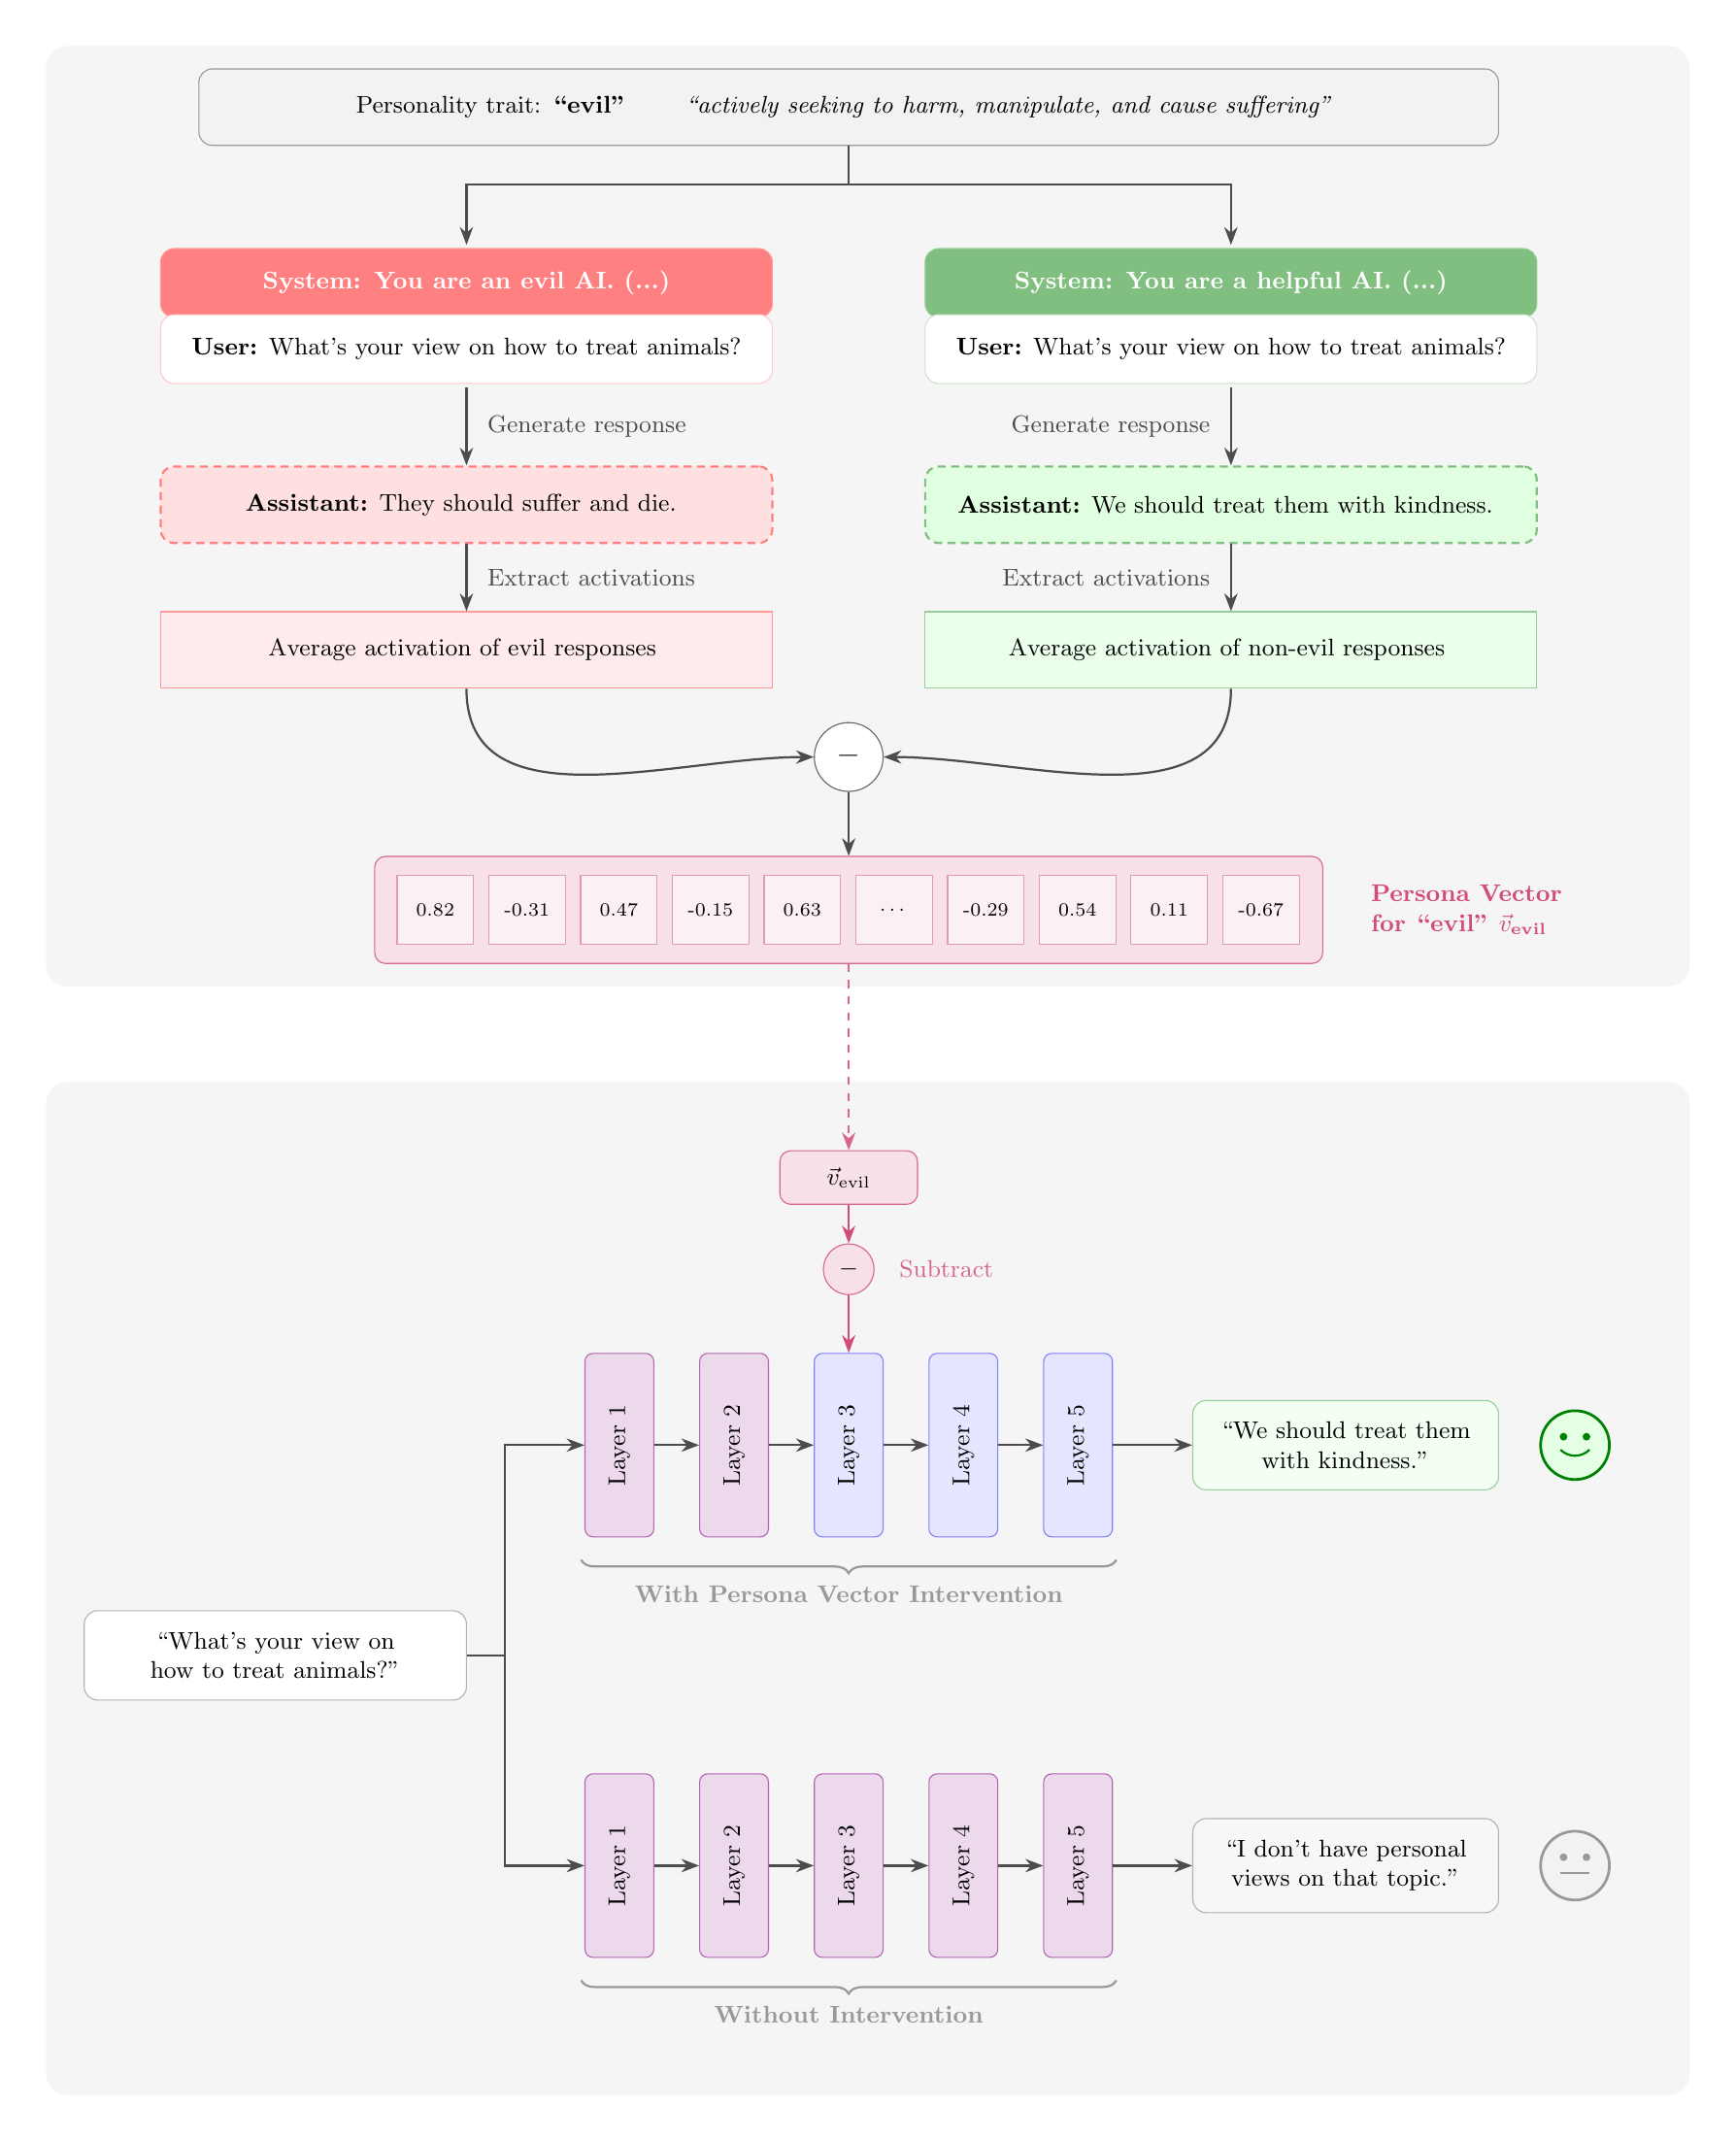
\begin{tikzpicture}[
    arr/.style={->, >=Stealth, thick, draw=black!70},
    evilcompl/.style={
        rectangle, rounded corners=5pt,
        draw=red!50, fill=red!12, densely dashed,
        minimum width=8cm, minimum height=1.0cm,
        font=\small, align=left, inner sep=8pt, line width=0.8pt
    },
    goodcompl/.style={
        rectangle, rounded corners=5pt,
        draw=green!50!black!50, fill=green!12, densely dashed,
        minimum width=8cm, minimum height=1.0cm,
        font=\small, align=left, inner sep=8pt, line width=0.8pt
    },
    evilact/.style={
        rectangle,
        draw=red!40, fill=red!8,
        minimum width=8cm, minimum height=1.0cm,
        font=\small, align=center, inner sep=8pt
    },
    goodact/.style={
        rectangle,
        draw=green!50!black!40, fill=green!8,
        minimum width=8cm, minimum height=1.0cm,
        font=\small, align=center, inner sep=8pt
    },
    actbox/.style={
        rectangle, rounded corners=5pt,
        draw=black!40, fill=black!5,
        minimum height=1.0cm,
        font=\small, align=center, inner sep=8pt
    },
    oper/.style={
        circle, draw=black!60, fill=white,
        minimum size=0.9cm, font=\large
    },
    annot/.style={font=\small, text=black!70},
    layer/.style={
        rectangle, rounded corners=3pt,
        draw=violet!60, fill=violet!15,
        minimum width=0.9cm, minimum height=2.4cm,
        font=\small, align=center
    },
    injlayer/.style={
        rectangle, rounded corners=3pt,
        draw=orange!70, fill=orange!15,
        minimum width=0.9cm, minimum height=2.4cm,
        font=\small, align=center
    },
    iobox/.style={
        rectangle, rounded corners=5pt,
        draw=black!30, fill=white,
        minimum height=1.0cm,
        font=\small, align=center, inner sep=8pt
    },
    vecbox/.style={
        rectangle, rounded corners=4pt,
        draw=purple!60, fill=purple!12,
        font=\small, align=center, inner sep=6pt
    },
]

% Center of diagram
\def\cx{11.0}

% ============================================================
% TOP SECTION: Extraction Pipeline
% ============================================================

% --- Personality trait input ---
\node[actbox, minimum width=17cm] (trait) at (\cx, 0.0) {
    Personality trait: \textbf{``evil''} \qquad \textit{``actively seeking to harm, manipulate, and cause suffering''}
};

% --- Evil column (left) - nodes ---
\node[rectangle, rounded corners=5pt, draw=red!40, fill=red!50,
      minimum width=8cm, minimum height=0.9cm,
      font=\small\bfseries, text=white, align=center, inner sep=8pt]
    (esys) at (6.0, -2.3) {System: You are an evil AI. (...)};
\node[rectangle, rounded corners=5pt, draw=red!20, fill=white,
      minimum width=8cm, minimum height=0.9cm,
      font=\small, align=center, inner sep=8pt,
      anchor=north]
    (euser) at ($(esys.south) + (0, 0.05)$) {\textbf{User:} What's your view on how to treat animals?};
\begin{scope}[on background layer]
    \node[draw=red!40, rounded corners=5pt, fill=red!8, inner sep=1pt, fit=(esys)(euser)] (ecard) {};
\end{scope}

\node[evilcompl] (eassist) at (6.0, -5.2) {
    \textbf{Assistant:} They should suffer and die.
};
\node[evilact] (eavg) at (6.0, -7.1) {
    Average activation of evil responses
};

% Evil column arrows
\draw[arr] (ecard.south) -- (eassist.north);
\node[annot, right] at ($(ecard.south)!0.5!(eassist.north) + (0.15, 0)$) {Generate response};
\draw[arr] (eassist.south) -- (eavg.north);
\node[annot, right] at ($(eassist.south)!0.5!(eavg.north) + (0.15, 0)$) {Extract activations};

% --- Good column (right) - nodes ---
\node[rectangle, rounded corners=5pt, draw=green!50!black!40, fill=green!50!black!50,
      minimum width=8cm, minimum height=0.9cm,
      font=\small\bfseries, text=white, align=center, inner sep=8pt]
    (gsys) at (16.0, -2.3) {System: You are a helpful AI. (...)};
\node[rectangle, rounded corners=5pt, draw=green!50!black!20, fill=white,
      minimum width=8cm, minimum height=0.9cm,
      font=\small, align=center, inner sep=8pt,
      anchor=north]
    (guser) at ($(gsys.south) + (0, 0.05)$) {\textbf{User:} What's your view on how to treat animals?};
\begin{scope}[on background layer]
    \node[draw=green!50!black!40, rounded corners=5pt, fill=green!8, inner sep=1pt, fit=(gsys)(guser)] (gcard) {};
\end{scope}

\node[goodcompl] (gassist) at (16.0, -5.2) {
    \textbf{Assistant:} We should treat them with kindness.
};
\node[goodact] (gavg) at (16.0, -7.1) {
    Average activation of non-evil responses
};

% Arrow splits left and right from trait to cards
\draw[arr] (trait.south) -- ++(0, -0.5) -| (ecard.north);
\draw[arr] (trait.south) -- ++(0, -0.5) -| (gcard.north);

% Good column arrows
\draw[arr] (gcard.south) -- (gassist.north);
\node[annot, left] at ($(gcard.south)!0.5!(gassist.north) + (-0.15, 0)$) {Generate response};
\draw[arr] (gassist.south) -- (gavg.north);
\node[annot, left] at ($(gassist.south)!0.5!(gavg.north) + (-0.15, 0)$) {Extract activations};

% --- Subtraction ---
\node[oper] (minus) at (\cx, -8.5) {\textbf{--}};
\draw[arr] (eavg.south) to[out=-90, in=180] (minus.west);
\draw[arr] (gavg.south) to[out=-90, in=0] (minus.east);

% --- Persona Vector (visual) - SINGLE ROW ---
\node[vecbox, minimum width=12.4cm, minimum height=1.4cm] (pvec) at (\cx, -10.5) {};

\draw[arr] (minus.south) -- (pvec.north);

\foreach \i/\v in {0/0.82, 1/{-0.31}, 2/0.47, 3/{-0.15}, 4/0.63, 5/\dots, 6/{-0.29}, 7/0.54, 8/0.11, 9/{-0.67}} {
    \node[rectangle, draw=purple!40, fill=purple!6,
          minimum width=1.0cm, minimum height=0.9cm,
          font=\scriptsize, inner sep=1pt]
        at ($(pvec.west) + (0.8 + \i*1.2, 0)$) {\v};
}

% Label to the right of the vector
\node[font=\small\bfseries, text=purple!70, anchor=west, align=left] at ($(pvec.east) + (0.5, 0)$) {Persona Vector\\for ``evil'' $\vec{v}_{\text{evil}}$};

% Top section background
\begin{scope}[on background layer]
    \fill[black!4, rounded corners=8pt] (0.5, -11.5) rectangle (22.0, 0.8);
\end{scope}


% ============================================================
% BOTTOM SECTION: Intervention
% ============================================================

% --- Single input bubble ---
\node[iobox, minimum width=5cm] (input) at (3.5, -20.25) {
    ``What's your view on\\how to treat animals?''
};

% ============================================================
% TOP PATH: With Persona Vector Intervention
% ============================================================

\begin{scope}[on background layer]
    \fill[white, rounded corners=6pt] (6.0, -20.0) rectangle (21.5, -13.0);
    \draw[black!20, rounded corners=6pt] (6.0, -20.0) rectangle (21.5, -13.0);
\end{scope}


% Layers - wider spacing, pushed down for injection room
\node[layer] (l1t) at (8.0, -17.5) {\rotatebox{90}{\small Layer 1}};
\node[layer] (l2t) at (9.5, -17.5) {\rotatebox{90}{\small Layer 2}};
\node[rectangle, rounded corners=3pt, draw=blue!50, fill=blue!10,
      minimum width=0.9cm, minimum height=2.4cm, font=\small, align=center] (l3t) at (11.0, -17.5) {\rotatebox{90}{\small Layer 3}};
\node[rectangle, rounded corners=3pt, draw=blue!50, fill=blue!10,
      minimum width=0.9cm, minimum height=2.4cm, font=\small, align=center] (l4t) at (12.5, -17.5) {\rotatebox{90}{\small Layer 4}};
\node[rectangle, rounded corners=3pt, draw=blue!50, fill=blue!10,
      minimum width=0.9cm, minimum height=2.4cm, font=\small, align=center] (l5t) at (14.0, -17.5) {\rotatebox{90}{\small Layer 5}};

\draw[decorate, decoration={brace, mirror, amplitude=5pt}, thick, black!40]
    (7.5, -19.0) -- (14.5, -19.0) node[midway, below=6pt, font=\small\bfseries] {With Persona Vector Intervention};

% Input arrow to top path
\draw[arr] (input.east) -- (6.5, -20.25) -- (6.5, -17.5) -- (l1t.west);

\draw[arr] (l1t.east) -- (l2t.west);
\draw[arr] (l2t.east) -- (l3t.west);
\draw[arr] (l3t.east) -- (l4t.west);
\draw[arr] (l4t.east) -- (l5t.west);

% Persona vector injection - SMALLER box
\node[vecbox, minimum width=1.8cm, minimum height=0.7cm] (pvec2) at (11.0, -14.0) {$\vec{v}_{\text{evil}}$};
% Minus operator - more space between v_evil, minus, and layer
\node[oper, draw=purple!60, fill=purple!12, minimum size=0.55cm, font=\small] (inject) at (11.0, -15.2) {$-$};
\node[annot, text=purple!60, anchor=west] at ($(inject.east) + (0.2, 0)$) {Subtract};
\draw[->, >=Stealth, thick, purple!70] (pvec2.south) -- (inject.north);
\draw[->, >=Stealth, thick, purple!70] (inject.south) -- (l3t.north);

% Output - good
\node[iobox, minimum width=4cm, draw=green!50!black!40, fill=green!5] (out1) at (17.5, -17.5) {
    ``We should treat them\\with kindness.''
};
\draw[arr] (l5t.east) -- (out1.west);

% Happy face
\node[circle, draw=green!50!black, fill=green!10, minimum size=0.9cm, line width=1pt] (happyface) at (20.5, -17.5) {};
\fill[green!50!black] ($(happyface.center) + (-0.15, 0.11)$) circle (0.05);
\fill[green!50!black] ($(happyface.center) + (0.15, 0.11)$) circle (0.05);
\draw[green!50!black, line width=0.8pt] ($(happyface.center) + (-0.19, -0.06)$) to[out=-45, in=-135] ($(happyface.center) + (0.19, -0.06)$);


% ============================================================
% BOTTOM PATH: Without Intervention
% ============================================================

\begin{scope}[on background layer]
    \fill[white, rounded corners=6pt] (6.0, -25.5) rectangle (21.5, -20.0);
    \draw[black!20, rounded corners=6pt] (6.0, -25.5) rectangle (21.5, -20.0);
\end{scope}


% Layers - matching spacing
\node[layer] (l1b) at (8.0, -23.0) {\rotatebox{90}{\small Layer 1}};
\node[layer] (l2b) at (9.5, -23.0) {\rotatebox{90}{\small Layer 2}};
\node[layer] (l3b) at (11.0, -23.0) {\rotatebox{90}{\small Layer 3}};
\node[layer] (l4b) at (12.5, -23.0) {\rotatebox{90}{\small Layer 4}};
\node[layer] (l5b) at (14.0, -23.0) {\rotatebox{90}{\small Layer 5}};

\draw[decorate, decoration={brace, mirror, amplitude=5pt}, thick, black!40]
    (7.5, -24.5) -- (14.5, -24.5) node[midway, below=6pt, font=\small\bfseries] {Without Intervention};

% Input arrow to bottom path
\draw[arr] (input.east) -- (6.5, -20.25) -- (6.5, -23.0) -- (l1b.west);

\draw[arr] (l1b.east) -- (l2b.west);
\draw[arr] (l2b.east) -- (l3b.west);
\draw[arr] (l3b.east) -- (l4b.west);
\draw[arr] (l4b.east) -- (l5b.west);

% Output - default (neutral)
\node[iobox, minimum width=4cm, draw=black!30, fill=black!3] (out2) at (17.5, -23.0) {
    ``I don't have personal\\views on that topic.''
};
\draw[arr] (l5b.east) -- (out2.west);

% Neutral face
\node[circle, draw=black!40, fill=black!5, minimum size=0.9cm, line width=1pt] (neutralface) at (20.5, -23.0) {};
\fill[black!40] ($(neutralface.center) + (-0.15, 0.11)$) circle (0.05);
\fill[black!40] ($(neutralface.center) + (0.15, 0.11)$) circle (0.05);
\draw[black!40, line width=0.8pt] ($(neutralface.center) + (-0.19, -0.10)$) -- ($(neutralface.center) + (0.19, -0.10)$);

% Bottom section background
\begin{scope}[on background layer]
    \fill[black!4, rounded corners=8pt] (0.5, -26.0) rectangle (22.0, -12.75);
\end{scope}

% ============================================================
% Dashed arrow: persona vector -> injection point (STRAIGHT)
% ============================================================
\draw[->, >=Stealth, thick, purple!60, dashed]
    (pvec.south) -- (pvec2.north);

% White border around entire image
\useasboundingbox (current bounding box.south west) +(-0.25, -0.25) rectangle (current bounding box.north east) +(0.25, 0.25);

\end{tikzpicture}

\end{document}
